\documentclass{whutmod}
\usepackage{metalogo}
\usepackage{enumitem}
\usepackage{graphicx}
\usepackage{subfigure}
\usepackage {mathtools}
\usepackage{algorithm}  
\usepackage{algorithmicx}  
\usepackage{algpseudocode}  
\usepackage{float}
\usepackage{listings}
\usepackage{color}
\usepackage{amsmath}%添加矩阵宏包
\graphicspath{{figures/}} %图片在当前目录下的figures还有目录picture下,还可以继续添加其他搜索路径
\definecolor{dkgreen}{rgb}{0,0.6,0}
\definecolor{gray}{rgb}{0.5,0.5,0.5}
\definecolor{mauve}{rgb}{0.58,0,0.82}
\definecolor{backcolour}{rgb}{0.95,0.95,0.95}
\lstset{frame=tb,
	language=Python,
	backgroundcolor=\color{backcolour},   
	aboveskip=3mm,
	belowskip=3mm,
	showstringspaces=false,
	columns=flexible,
	basicstyle={\small\ttfamily},
	numbers=none,
	numberstyle=\tiny\color{gray},
	keywordstyle=\color{blue},
	commentstyle=\color{dkgreen},
	stringstyle=\color{mauve},
	breaklines=true,
	breakatwhitespace=true,
	tabsize=3
}
%插入参考文献命令
\newcommand{\upcite}[1]{\textsuperscript{\textsuperscript{\cite{#1}}}}

\renewcommand{\algorithmicrequire}{\textbf{Input:}}  % Use Input in the format of Algorithm  
\renewcommand{\algorithmicensure}{\textbf{Output:}} % Use Output in the format of Algorithm  
\team{026}	% 组号
\membera{许鸢飞}
\joba{编程}
\memberb{尹可汗}
\jobb{编程写作}
\memberc{李想}
\jobc{建模写作}
\title{xxxx}
\tihao{3} % 题号

\begin{document}

\maketitle
%摘要
\begin{abstract}
	\keywords{
		xxx \quad
		xxx \quad
	}
\end{abstract}

\tableofcontents
\newpage

%绘制普通三线表格 
%
%表格应具有三线表格式,因此常用 booktabs宏包,其标准格式如表~\ref{tab001}~所示。
%\begin{table}[!htbp]
%	\caption{标准三线表格}\label{tab001} \centering
%	\begin{tabular}{ccccc}
%		\toprule[1.5pt]
%		$D$(in) & $P_u$(lbs) & $u_u$(in) & $\beta$ & $G_f$(psi.in)\\
%		\midrule[1pt]
%		5 & 269.8 & 0.000674 & 1.79 & 0.04089\\
%		10 & 421.0 & 0.001035 & 3.59 & 0.04089\\
%		20 & 640.2 & 0.001565 & 7.18 & 0.04089\\
%		\bottomrule[1.5pt]
%	\end{tabular}
%\end{table}
%\section{例子}
%\subsection{引用}
%引言 \upcite{knuth86a}
%
%\begin{itemize}
%	\item item1 \upcite{deng:01a}
%	\item item2
%	\item item3
%\end{itemize}
%
%
%\subsection{行内公式}
%
%行内公式$i=0,1,...n$。
%独占一行的公式$$E(P) = {a_1}{P^3} + {a_2}{P^2} + {a_3}P + {a_4},$$
%
%\subsection{公式自动编号}
%
%自动编号的公式
%\begin{equation}
%	\label{myeqname1}
%	p_{j}=\begin{cases} 0,&\text{if $j$ is odd}\\
%	r!\,(-1)^{j/2},&\text{if $j$ is even}
%	\end{cases}
%\end{equation}
%
%
%\begin{equation}
%	\label{myeqname2}
%	\arcsin \theta  =
%	\mathop{{\int\!\!\!\!\!\int\!\!\!\!\!\int}\mkern-31.2mu
%		\bigodot}\limits_\varphi{\mathop {\lim }\limits_{x \to \infty } \frac{{n!}}{{r!\left( {n - r}\right)!}}}
%\end{equation}
%\subsection{公式引用}
%由(\ref{myeqname2})式。
%
%\subsection{图片引用}
%
%流程见图\ref{T0-0}。
%\begin{figure}[!htbp]
%	\centering
%%	\includegraphics[width=.95\textwidth]{figures/Mind_mapping1.png}
%	\caption{问题一思维导图}
%	\label{T0-0}
%\end{figure}
%
%画统计类图表都使用Python的matplotlib.pyplot库,保存为矢量图(pdf)格式。画图独立定义一个文件plot.py,导包过程和画图函数模板如下。
%\begin{lstlisting}[language=python]
%import matplotlib.pyplot as plt
%from matplotlib.backends.backend_pdf import PdfPages# 支持保存pdf矢量图
%
%def plot_map(station, save=True, pointSize=25, name="map"):
%	# print(station["classID"])
%	plt.figure()
%	plt.scatter(station["X"], station["Y"], s=pointSize-10*station["classID"], c=station["classID"], cmap="Set1")
%	plt.xlabel("X (km)")
%	plt.ylabel("Y (km)")
%	if save:
%		pdf = PdfPages("img//{}.pdf".format(name))
%		pdf.savefig()
%		pdf.close()
%	else:
%		plt.show()
%	plt.close()
%
%\end{lstlisting}

\section{问题重述}
\subsection{问题背景}

信息的生成,获取,传输是网络连通环节的重要组成部分,随着现代无线充电技术,快速充电技术等的迅速发展,无线传感器网络受到了越来越多的关注.无线传感器网络是一个复杂的系统,由传感器,处理器,无线通信和能量供应三个模块组成,传感器模块用以接受外界数据信息并将其发送至处理器模块,处理器模块对信息进行处理并储存,由无线通信模块进行信息的收发.
无线可充电传感网络WRSN(Wireless Rechargeable Sensor Network)已经被大量应用于天气信息收集,电子信号收发等任务中.无线可充电网络的示意图如\ref{示意图}
\begin{figure}[!htbp]
	\centering
	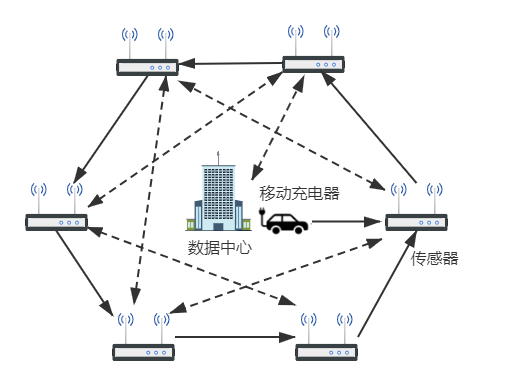
\includegraphics[width=0.6\textwidth]{system.png}
	\caption{无线可充电网络示意图}
	\label{示意图}
\end{figure} 




\subsection{待解决的问题}
\textbf{问题一:}对一般性的路径规划问题进行研究,给出WRSN充电规划模型和相应的求解算法.算出充电器在路上的最小能量消耗以及相应路线.

\textbf{问题二:}利用表二给出的3组参数,通过增加约束条件:充电器的充电,移动以及传感器的能量消耗限制,求出在指派单一充电车的情况下,系统内各传感器需要的最小电池容量。

\textbf{问题三:}对于多充电车路径优化模型,给出相应算法求解出系统最小总能量消耗,并求出每个传感器的最小电池容量。


\section{模型假设}
\begin{enumerate}
	\item 假设每次充电时,充电器一定会将传感器电充满再离开,防止出现充电不完全的状态。
	\item 假设小车移动过程中呈匀速运动,忽略启动和停车的加速度影响。
\end{enumerate}


\section{符号说明}
\begin{center}
	\begin{tabular}{ccccc}
		\toprule[1.5pt]
		符号 & 含义\\
		\midrule[1pt]
		$C$ & 移动充电器集合\\
		$O$& 数据中心的集合\\
		$M$& 表示传感器的集合\\
		$m_0,m_{1..29}$ &表示数据中心和传感器的元素\\
		$d_{ij}$&表示节点$i$和节点$j$之间的距离\\
		$f$ & 传感器电量的最低阈值\\
		$v$ & 移动充电器移动速率\\
		$r$ & 移动充电器的充电速率\\
		$T_1$&小车在数据中心的休息时长\\
		\bottomrule[1.5pt]
		注:表中未说明的符号以首次出现处为准
	\end{tabular}
\end{center}




\section{问题一模型的建立与求解}
\subsection{问题分析}
问题给出了WRSN系统中传感器的经纬度坐标位置,需要首先进行转化以求出传感器,数据中心间的两两距离,而在充电车对每个传感器充电是正常且必需的,那么要使得该充电器能量消耗最小,则必须使得充电器在路上的能量消耗最少即就是路径最少,在指派单一充电车的情况下,则该问题可转化为一个简单旅行商问题(TSP问题),所以我们可以采用组合优化的思想,通过组合优化路径规划模型来求解该问题。
\begin{figure}[!htbp]
	\centering
	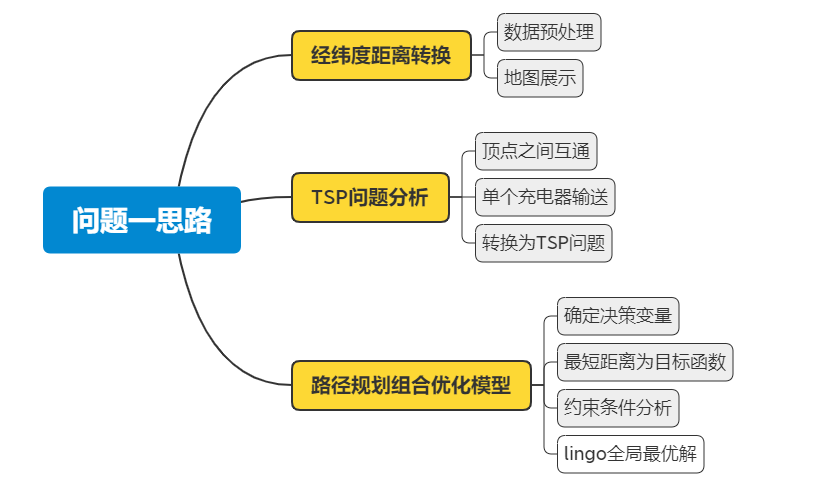
\includegraphics[width=.6\textwidth]{figures/mindmap1.png}
	\caption{问题一思维导图}
\end{figure} 
%插入参考文献\upcite{bib:one}。

\subsection{数据预处理}
为了得到传感器,数据中心两两之间的路径距离,我们需要对经纬度进行转换.

地球上任意一点的地理坐标都可以用有序数对(u,v),u,v分别表示经度和维度。以地心O为坐标原点,赤道平面为$xOy$平面,0度经线圈所在的平面为$xOZ$平面建立三维直角坐标系,则

\begin{equation}\left\{\begin{array}{l}
		x=R \cos u \cos v .\\
		y=R \sin u \cos v .\\
		z=R \sin v.
	\end{array}\right.
\end{equation}

其中,$R=6370$为地球半径.
任意两点$A$($u_{A}$,$v_{A}$),$B$($u_{B}$,$v_{B}$)间的实际距离为

\begin{equation}
	d=R \arccos( \frac{OA\times OB}{|OA|\times |OB|}).
\end{equation}

综合(1)(2)式得

\begin{equation}
	d=R \arccos \left[\cos (u_{A}-u_{B})\cos v_{A} \cos v_{B}+\sin v_{A} \sin v_{B}\right].
\end{equation}

\subsection{单一充电器路径规划组合优化模型}
在题中要求无线可充电传感器网络WRSN需要外界传导能量以维持运行,为此移动充电器需要定期为传感器进行充电以避免其电量低于阈值。移动充电器从数据中心出发,以固定的速度依次经过每个传感器,在每个传感器处停留一段时间并以固定的充电速率为传感器充电,直到为所有传感器充电完成之后返回数据中心,由于传感器之间,传感器与数据中心之间都存在一条通路,而且只有一个单一充电器供能,所以该问题可以转换成一个旅行商问题,利用组合优化的方法来解决。
\begin{figure}[!htbp]
	\centering
	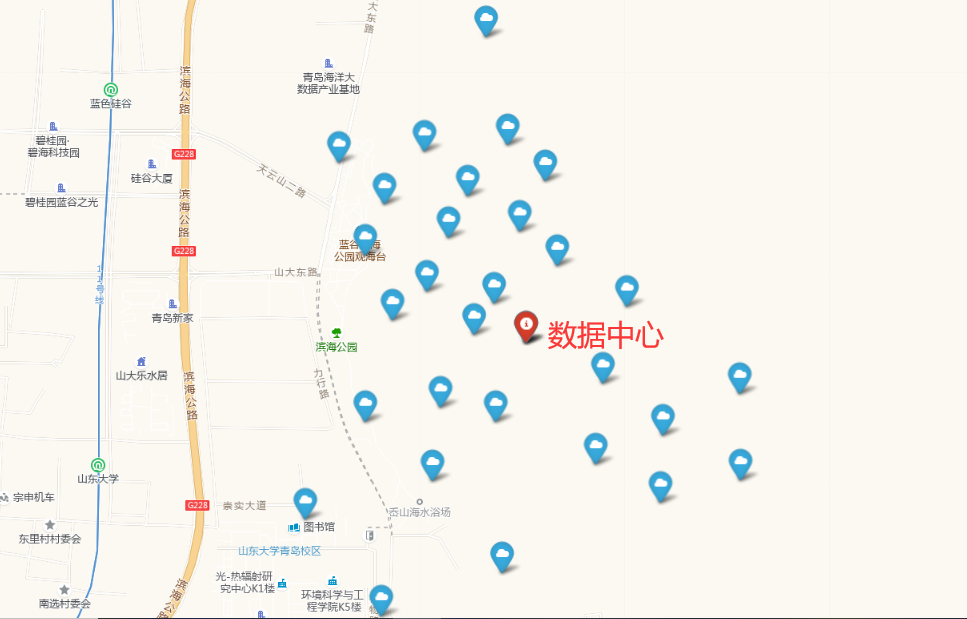
\includegraphics[width=.6\textwidth]{figures/origin.png}
	\caption{各节点经纬度所在原始区域地图}
\end{figure} 
\subsubsection{决策变量}
设数据中心为$O$点集合内包含$\{m_0\}$,充电车集合$C= \{c_{1}\}$,接收器集合$M=\{m_{1},m_{2},m_{3}....m_{29}\}$.
这里我们引入01变量.

%\begin{equation}
%	\label{myeqname1}
%	p_{j}=\begin{cases} 0,&\text{if $j$ is odd}\\
%	r!\,(-1)^{j/2},&\text{if $j$ is even}
%	\end{cases}
%\end{equation}
\begin{equation}
	x_{ij}=\begin{cases} 
		0,&\text{$m_i$和$m_j$存在路径.} \\
		1,&\text{$m_i$和$m_j$不存在路径.} \\
	\end{cases}
\end{equation}


\subsubsection{目标函数}
充电车从数据中心出发,依照一定顺序经过所有接收点,任意两接收点有一确定的道路连通.我们通过(3)式求出接收器两两之间的距离
$d_{ij}$表示接收器$i$与$j$之间的距离,$(0<i,j\leq n )$
\begin{equation}
	d_{ij}=R \arccos \left[\cos (u_{i}-u_{j}) \cos v_{i} \cos v_{j}+\sin v_{i} \sin v_{j}\right].
\end{equation}
\begin{equation}
	\min Length=\min\sum_{i=1}^{n}\sum_{j=1}^nd_{ij}x_{ij}.
\end{equation}

\subsubsection{约束条件}
保证每个传感器节点后只有一个节点与其想连通,即节点出度为1
\begin{equation}
	\sum_{j=1}^{n} x_{ij} = 1,i=1,2...n.
\end{equation}

保证每个传感器节点前只有一个节点与其想连通,即节点入度为1
\begin{equation}
	\sum_{i=1}^{n} x_{ij} = 1,i=1,2...n.
\end{equation}

为防止产生多于1个的连通回路,且保证每个结点都将连通构成回路,引入该节点边数与传感器之间编号构成的联系。
\begin{equation}
	m_i-m_j+nx_{ij}\le n-1,1<i\ne j\le n.
\end{equation}

保证出去回到节点的边以后,所构成的路径边数满足树的边数构造即等于顶点数n-1。
\begin{equation}
	\sum_{i,j\in S}x_{ij}\leq |S|-1,2\leq |S|\leq n-1, S\in(1,2,....n.).
\end{equation}

\subsubsection{模型汇总}
综上所述,我们建立了以最短移动路径$\min Length$为目标函数,节点出度和入度为1,回路限定等条件,建立了用于解决单一充电器路径规划旅行商问题的组合优化模型。
\begin{equation}
	\min Length=\min\sum_{i=1}^{n}\sum_{j=1}^nd_{ij}x_{ij}.
\end{equation}

\begin{equation}
	s.t.
	\begin{cases} 
		\sum_{j=1}^{n} x_{ij} = 1,&i=1,2...n.\\
		\sum_{i=1}^{n} x_{ij} = 1,&i=1,2...n.\\
		\sum_{i,j\in S}x_{ij}\leq $|S|$-1,& 2\leq |S|\leq $n$-1, S\in(1,2,....n.).\\
		m_i-m_j+nx_{ij}\le n-1,1<i\ne j\le n, & 1<i\ne j\le n. \\
		x_{ij}=0 \quad or \quad 1,& i,j=1,..n.\\
		m_i \in O \cup M,& i=1,..n.
	\end{cases}
\end{equation}
%\begin{figure}[!h]
%	\centering
%	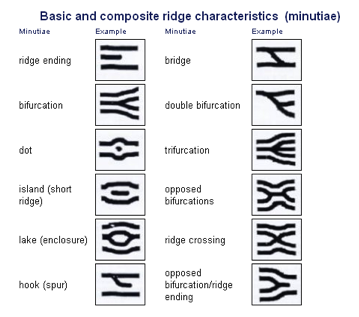
\includegraphics[width=0.8\textwidth]{class.png}
%	\caption{细节点类型示意图}
%	
%\end{figure}



%\begin{equation}
%M_{i}=\frac1{WH}\sum_{i=0}^{H-1}\sum_{j=0}^{W-1}I(i,j)
%\end{equation}
%\begin{equation}
%V_{i}=\frac1{WH}\sum_{i=0}^{H-1}\sum_{j=0}^{W-1}({I(i,j)-M_{i})^2}
%\end{equation}

%
%\begin{equation}
%$$ $$
%\end{equation}




%\begin{tabular}{|c|c|c|c|c|c|c|c|c|c|r|}
%	\hline
%	$\delta$$x_{1}$ & $\delta$$ y_{1}$ & $t_{1}$ & $k_{1}$ & $\delta$$ x_{2}$ & $\delta $$y_{2}$ & $t_{2}$ & $k_{2}$ & ... & $t_{20}$ & $k_{20}$\\
%	\hline
%\end{tabular}
\subsection{模型求解}
\textbf{step1:}我们将该问题的经纬度利用地球半径和球面的计算公式求得了整个区域各顶点之间的距离矩阵$D$。
\begin{equation}
	D=\begin{bmatrix}
		d_{00} & \dots & d_{0n} \\
		\vdots & \ddots & \vdots \\
		0 & & d_{nn}
	\end{bmatrix}_{n \times n}
\end{equation}
\begin{figure}[!h]
	\centering
	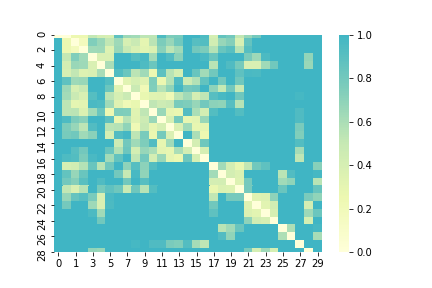
\includegraphics[width=0.7\textwidth]{heatmap1.pdf}
	\caption{各节点构成的距离矩阵}
\end{figure}

\textbf{step2:}采用lingo编程,将得到的距离矩阵$D$中的元素带入目标函数$\min Length$和上述约束条件中。从该问题的类型和规模上来看,该问题的数据和规模较小,而且求解的目标函数简单唯一,且需要得到全局最优解,本文采用lingo能够快速高效的解决该问题,将给定的约束条件和模型输入即得到了正确的结果。
\subsection{结果分析}
\subsubsection{结果展示}
通过lingo程序的高效计算,我们得到了该问题的全局最优解,求得该移动充电器的全局最短路径$\min Length=11.48276km$
\begin{figure}[!h]
	\centering
	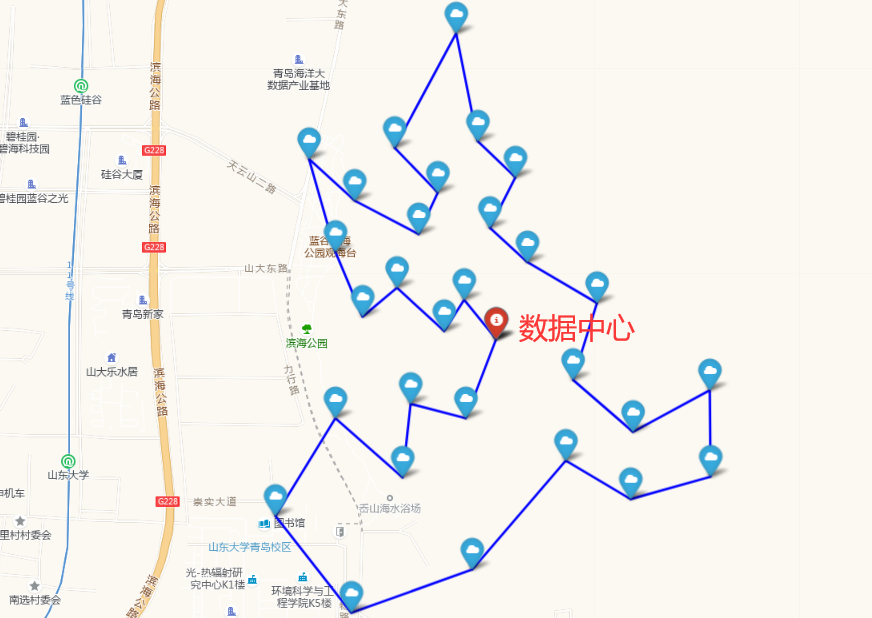
\includegraphics[width=0.7\textwidth]{route1.png}
	\caption{单一充电器路线规划图}
\end{figure}

\begin{table}[!htbp]
	\caption{问题一路径详细过程} \centering
	\begin{tabular}{c}
		\toprule[1.5pt]
		编号详细路径 \\
		\midrule[1pt]
		$m_0\text{(数据中心)}->m_2->m_1->m_9->m_7->m_6->m_{14}->m_{11}->m_8->m_{12}->$ \\
		$m_{15}->m_{27}->m_{16}->m_{13}->m_{10}->m_{5}->m_{3}->m_{4}->m_{22}->m_{28}->$\\
		$m_{24}->m_{23}->m_{21}->m_{29}->m_{26}->m_{25}->m_{18}->m_{19}->m_{20}->m_{17}->m_0$\\
		\bottomrule[1.5pt]
	\end{tabular}
\end{table}
%\subsubsection{灵敏度分析}

\section{问题二模型的建立与求解}
\subsection{问题分析}
问题二要求我们在第一问求得的最短路径的基础上,算出个传感器携带的电池容量大小.需考虑到传感器的工作能量损耗$P$和电量阈值$f$限制,充电小车的运行速度$v_{c}$以及充电速度$r$对整个无线传感器网络工作的影响.

问题二的思维导图如\ref{mindmap2} 所示
\begin{figure}[!h]
	\centering
	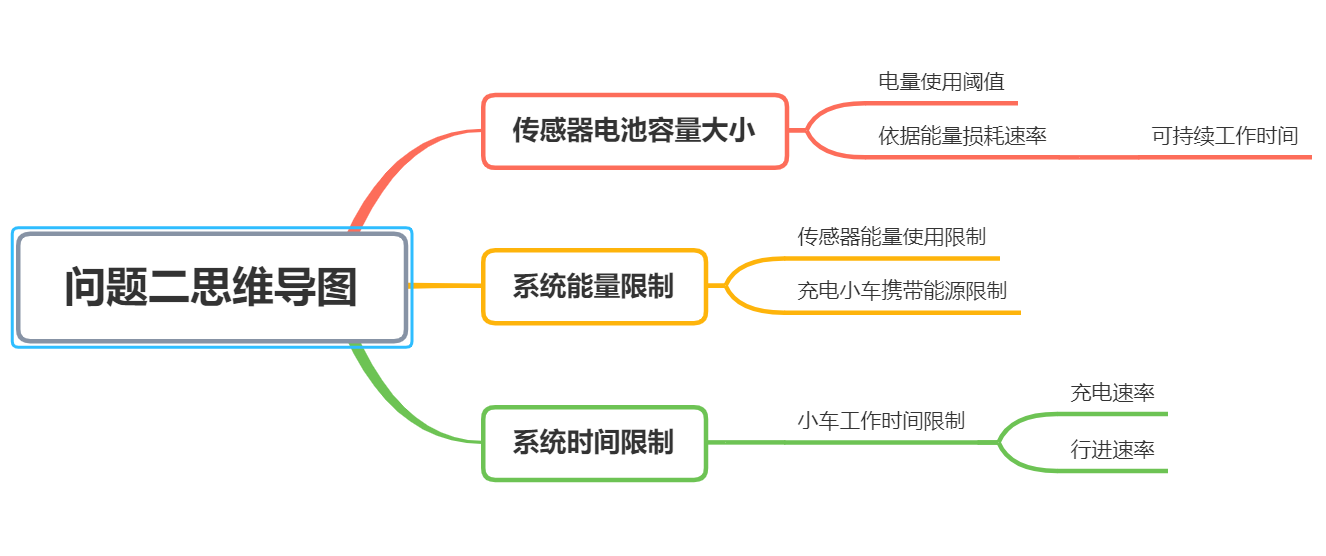
\includegraphics[width=0.8\textwidth]{mindmap2.png}
	\caption{问题二思维导图}
	\label{mindmap2}
\end{figure}
\subsection{能量和时间约束的传感器容量设计模型}
传感器电池的设计容量大小会受到电量使用阈值和能量损耗速度的限制,单个传感器由于处在一个多节点构成的系统中,为此还要受到整个系统运行周期的限制,为此我们建立了一个多重线性约束模型.
\subsubsection{决策变量}
充电小车在系统内工作的时间内,可以认为控制其在数据中心的休息时间.如果进行小车的轮换,则可以保证系统在任意时间内都有一辆小车正在运行.如果在数据中心内对小车进行充电,则可以调整小车的休息时间.
\begin{equation}
	T_{1}=\begin{cases} 
		0,&\text{小车不进行休息.} \\
		t,&\text{小车在数据中心修整t的时长}. \\
	\end{cases}
\end{equation}


\subsubsection{目标函数}
根据小车运行一圈的时间与小车和传感器的设定参数,从时间和能量两个方面建立了能量和时间约束的传感器容量设计模型.
\begin{equation}
	\min e_{nmax}=f_{n}+p_{n}\times T^{\prime}.
\end{equation}

$e_{nmax}$表示的是第n个传感器的最大容量设计,$f_{n}$表示的是第n个传感器工作的最低阈值(mA/h),$p_{n}$是第n个传感器的消耗速率,$T^{\prime}=T+T_{1}$表示该小车工作一圈的时间和休息的时间之和,代表小车的运行过程中一圈的时间周期。
\subsubsection{约束条件}
\textbf{能量约束}

无论是充电小车和传感器都会受到能源使用限制,传感器受到的限制来自使用电量的阈值限制和传感器能量消耗限制,小车则受到携带能量大小的限制.
\begin{equation}
	\left\{\begin{array}{l}
		e_{ncu} \geq f_{n},\quad n=1,2,...29.\\
		f_{n}=ke_{nmax}.\\
		\sum_{i=1}^{n} e_{nmax}-e_{ncu}+E_{c} \leq E_{max}.\\
		E_{c} =\sum_{i\neq j}(\frac{d_{ij}}{v_{c}}) \times g_{c}.
	\end{array}\right.
\end{equation}

式中:$e_{ncu}$表示编号为n的传感器现有电量值,$f_{n}$为编号为n的传感器的能量阈值,k为一比例系数,表示阈值与设计容量的比例.$e_{nmax}$表示编号为n的传感器的能量设计容量.$E_{c}$表示充电车在路上的能量消耗,与充电车行进的时间有关,行进过程中由于动力消耗能量的功率为$g_{c}$.

\textbf{时间约束}

传感器的有效使用时间$t_{n}$指的是传感器从充满电状态变为能量接近阈值状态所经过的时间,其大小需大于充电周期的时长$T^{\prime}$,而小车在系统内运行一周的时间取决于行进耗费的时间和为传感器充电耗费的时间.

\begin{equation}\left\{\begin{array}{l}
		T^{\prime}=T+T_{1} .\\
		T=\sum_{i\neq j}(\frac{d_{ij}}{v_{C}})+\sum_{i=1}^{n} \frac{e_{nmax}-e_{ncu}}{r}. \\	
		\min {t_{n}} \ge T^{\prime}.\\
		t_{n}=\frac{e_{nmax}-f_{n}}{p_{n}}.
	\end{array}\right.
\end{equation}

式中: $T_{1}$为充电车在数据中心充电时间,$p_{n}$为编号为n的传感器的能量损耗速度.\qquad r为充电车给传感器的充电速度.

\subsubsection{模型汇总}
综上所述,我们从时间和空间两个方向的约束,通过查阅相关资料的参数设定,在问题一的路径规划基础上建立了一个传感器容量设定的模型。
\begin{equation}
	\min e_{nmax}=f_{n}+p_{n}\times T^{\prime}.
\end{equation}

\begin{equation}\left\{\begin{array}{l}
		e_{max}=\frac {p_{n}\times (T+T_{1})}{1-K}.\\	
		T=\frac{\sum_{i=1}^{n}p_{n}T_{1}+r\sum_{i\neq j}(\frac{d_{ij}}{v_{c}})} {r-\sum_{i=1}^{n}p_{n}}.\\
		
	\end{array}\right.
\end{equation}

\subsection{参数估计}
通过查阅相关文献资料\upcite{bib:one}\upcite{bib:two}\upcite{bib:three}我们对系统内相关参数进行设置,具体参数范围如表\ref{canshu2}

\begin{table}[!htbp]
	\caption{参数估计表}\label{canshu2} \centering
	\begin{tabular}{cc}
		\toprule[1pt]
		名称 & 参数范围\\
		\midrule[1pt]
		充电速率& 3-5$J/s$\\
		小车运行速度$v$& 3-5$m/s$\\
		能量阈值系数$k$& 20\%-30\% \\
		传感器能量消耗速度$p_{n}$ &3.5-7.8$mA/h$ \\
		传感器电压&10-24$V$\\		
		\bottomrule[1.5pt]
	\end{tabular}
\end{table}

\subsection{结果分析}
\subsubsection{结果展示}
我们首先对所有参数指标取范围的平均值以估算传感器设计电池容量.在充电速率$r$取4焦耳每秒,小车运行速度$v_{c}$取4$m$/s,能量阈值系数取25\%.传感器电压取17伏特.带入(19)式,求解得:$T=4.04$小时.系统一个周期运行的时间$T^{\prime}$为5.04小时.如果需要统一传感器规格,则根据系统内电池容量要求最大的传感器选择电池容量设计大小,为52.4瓦时.



\begin{table}[!htbp]
	\caption{各个小车容量设计}\label{canshu2} \centering
	\begin{tabular}{cccccccccc}
		\toprule[1pt]
		编号 & 容量 & 编号 & 容量 & 编号 & 容量 & 编号 & 容量 & 编号 & 容量\\
		\midrule[1pt]
		1 & 36.3  & 7 & 43.0 & 13 & 43.7 & 19 &  37.0 & 25 & 50.4\\
		2 & 52.4 & 8 &  30.9 & 14 & 30.2 & 20 & 30.2 & 26 & 28.9\\
		3 & 30.2 & 9 &  30.2 & 15 & 25.5 & 21 &  37.0 &27 & 24.1\\
		4 & 36.7 & 10 &  37.0 & 16 & 30.2 & 22 & 30.2 & 28 & 43.0\\
		5 & 24.2 & 11 &   30.2 & 17 & 25.5 & 23 & 23.5 & 29 & 36.3\\
		6 & 30.2 & 12 &   49.7 & 18 & 30.2 & 24 & 37.0  & /  & / \\
		\bottomrule[1.5pt]
	\end{tabular}
	\centering
\end{table}

\subsubsection{参数分析}
我们发现小车运行速度与传感器充电功率大小与传感器设计最小容量呈负相关,而小车的休息时间长短与传感器电压大小与传感器设计最小容量呈正相关.
从直观的角度分析,小车的前进速率越快,充电效率越高,每一圈运行的时间就越短,传感器电池容量要求就会越小.而小车休息市场越长则是变相延长了传感器的可持续使用时间,传感器电压越高,释放的能力就越多,对传感器电池容量的要求就越高.所以我们的结果是符合逻辑的.
我们画出了该系统中传感器电池设计的最小容量随4种参数数值变化的图像。

\begin{figure}[H]	
	\begin{minipage}[t]{0.48\textwidth}
		\centering
		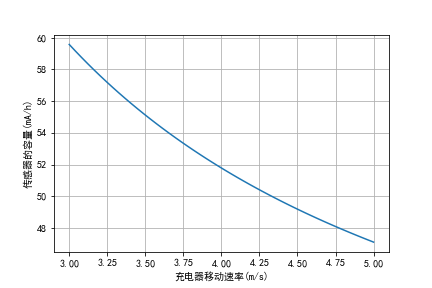
\includegraphics[width=0.99\textwidth]{speed.png}	
		
		\caption{小车运行速度的影响}
	\end{minipage}
	\qquad
	\begin{minipage}[t]{0.48\textwidth}
		\centering
		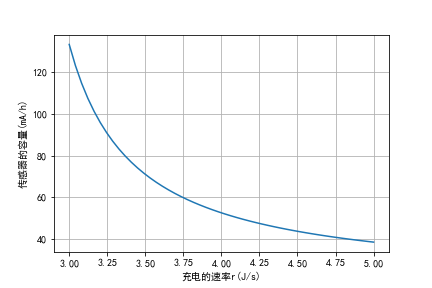
\includegraphics[width=0.99\textwidth]{chargeSpeed.png}
		
		\caption{传感器充电功率的影响}	
	\end{minipage}
	\label{fig:enhance}
	
\end{figure}
\begin{figure}[H]	
	\begin{minipage}[t]{0.48\textwidth}
		\centering
		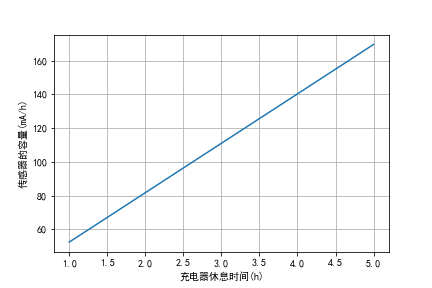
\includegraphics[width=0.99\textwidth]{breakTimg.png}	
		
		\caption{充电小车休息时间的影响}
	\end{minipage}
	\qquad
	\begin{minipage}[t]{0.48\textwidth}
		\centering
		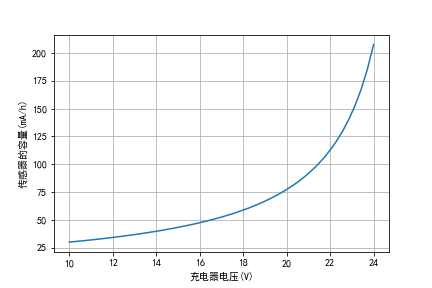
\includegraphics[width=0.99\textwidth]{V.png}
		
		\caption{传感器电压的影响}	
	\end{minipage}
	\label{fig:enhance}
	
\end{figure}

对传感器设计电池容量大小影响最大的因素是小车的休息时间,小车休息时间每多增加一个小时,则会使传感器电池最小容量增加29.2毫安时.相对于其他因素来说,小车运行速度对传感器电池容量大小的影响最小,我们认为这是因为在小车在路径上行驶的时间只占系统周期性运行时间的一小部分,而充电小车给传感器充电的时间则相对更长,图7和图8也验证了我们的猜想.

图10显示传感器的电压对传感器电池容量影响较大,要注意的是,传感器的电压常常是一个确定值,在传感器设计师就已经确定了.所以为了控制电池容量,应尽可能提高传感器性能,使其在相对低压环境下工作.


\section{问题三模型的建立与求解}
\subsection{问题分析}
问题三要求我们在问题一的单充电车路径规划的基础上,思考为提高充电效率而派出4台移动充电车时,如何规划移动充电器的路径以使得移动充电器在路上的总能量消耗最少,即求出移动充电器形势的最短路径,这实际上是一个含载重量的车辆路径问题(CVRP),CVRP是TSP的一种推广。
是一个仓库,应该创建多条路径,每条路径的起点和终点都在仓库。
同时由于充电器仍需满足问题二中提到的能量约束和时间约束,我们可以相应的求出各个路径上不同的传感器设计容量大小.

\subsection{注意力模型的建立}
注意力模型(Attention Model)被广泛应用于自然语言处理,图像识别及语音识别等各种不同类型的深度学习任务中.
目前绝大多数文献中出现的注意力模型是依附在编码器-解码器框架下的.解码器-编码器框架(图\ref{kuangjia})可以看做是一种文本或数据处理领域的研究模式.
\begin{figure}[!h]
	\centering
	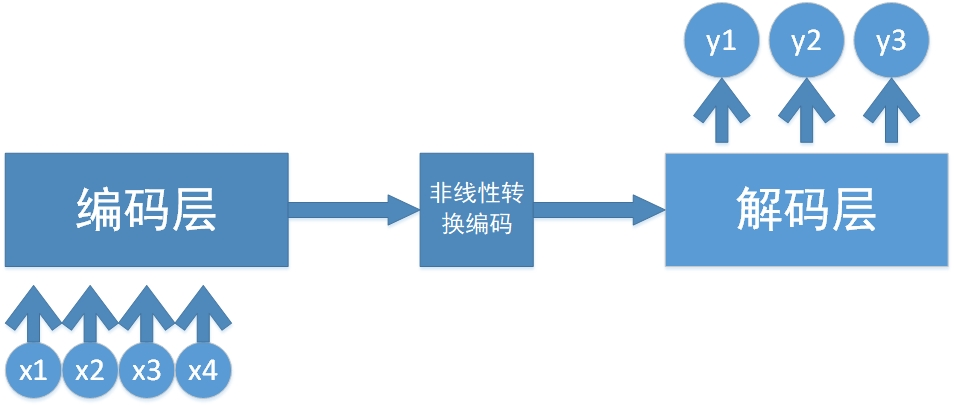
\includegraphics[width=0.45\textwidth]{framework.jpg}
	\caption{框架示意图}
	\label{kuangjia}
\end{figure}

\subsubsection{编码器}
我们使用的编码器类似于Vaswani\upcite{bib:four}等人在Transformer体系结构中使用的编码器,但是我们不使用位置编码,产生的节点嵌入对输入的顺序是不变的.输入二维特征$x_{i}$,编码器同过具有参数$W^{X}$和$b^{x}$的学习线性投影计算初始二维节点嵌入$h_{i}^{(0)}$.
\begin{equation}
h_{i}^{(0)}.=W^{X}x_{i}+b^{x}.
\end{equation}
 嵌入后使用$N$个注意层进行更新,每个注意层由两个子层组成,我们用$h_{i}^{(\ell )}$表示由$\ell$层产生的节点嵌入, 编码器计算输入图的聚合嵌入$\overline h^{(N)}$作为最终节点嵌入$h_{i}^{(N)}$的平均值.
\begin{equation}
\overline h^{(N)}=\frac{1}{n}\sum_{i=1}^{n}h_{i}^{(N)}
\end{equation}
节点嵌入$h_{i}^{(N)}$和图嵌入$\overline h^{(N)}$都被用作解码器的输入.

\textbf{Attention layer}\quad 遵循Transformer架构如图\ref{fig:encoder}。 每个注意层由两个子层组成: 一种多头注意层(MHA),执行节点和节点上完全连接的前馈层(FF)之间的消息传递。每个子层增加skip-connection和batch nomrmlization。
\begin{equation}
\hat{\mathbf{h}}_{i} =\mathrm{B} \mathrm{N}^{\ell}\left(\mathbf{h}_{i}^{(\ell-1)}+\mathrm{MHA}_{i}^{\ell}\left(\mathbf{h}_{1}^{(\ell-1)}, \ldots, \mathbf{h}_{n}^{(\ell-1)}\right)\right) \\
\end{equation}
\begin{equation}
\mathbf{h}_{i}^{(\ell)} =\mathrm{B} \mathrm{N}^{\ell}\left(\hat{\mathbf{h}}_{i}+\mathrm{FF}^{\ell}\left(\hat{\mathbf{h}}_{i}\right)\right)
\end{equation}
每层的索引$\ell$表示图层不共享参数。
\begin{figure}[!h]
	\centering
	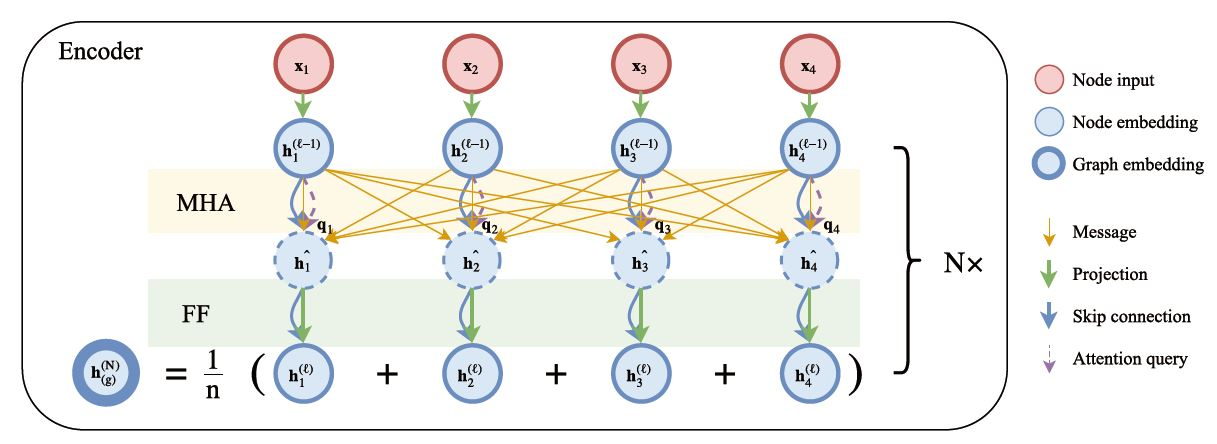
\includegraphics[width=0.6\textwidth]{encoder.jpg}
	\caption{编码器示意图}
	\label{fig:encoder}
\end{figure}

\subsubsection{解码器}
解码器按照顺序解码,按照时间步长$t\in {1,...n}$, 解码器基于编码器的嵌入输出节点$\pi_{t}$,在步长$t^{\prime}<t$时输出$\pi_{t^{\prime}}$

\textbf{内容嵌入}\quad
解码器在时间$t$的内容来自编码器和输出的内容.对于TSP问题,它由前一个节点$\pi_{t-1}$和第一个节点$\pi_{1}$的嵌入构成.对于$t=1$时, 我们使用学习的$d_{h}$维参数$v^{l}$和$V^{f}$作为输入占位符:
\begin{equation}\mathbf{h}_{(c)}^{(N)}=\left\{\begin{array}{ll}
{\left[\overline{\mathbf{h}}^{(N)}, \mathbf{h}_{\pi_{t-1}}^{(N)}, \mathbf{h}_{\pi_{1}}^{(N)}\right]} & t>1 \\
{\left[\overline{\mathbf{h}}^{(N)}, \mathbf{v}^{1}, \mathbf{v}^{f}\right]} & t=1
\end{array}\right.\end{equation}

\begin{figure}[!h]
	\centering
	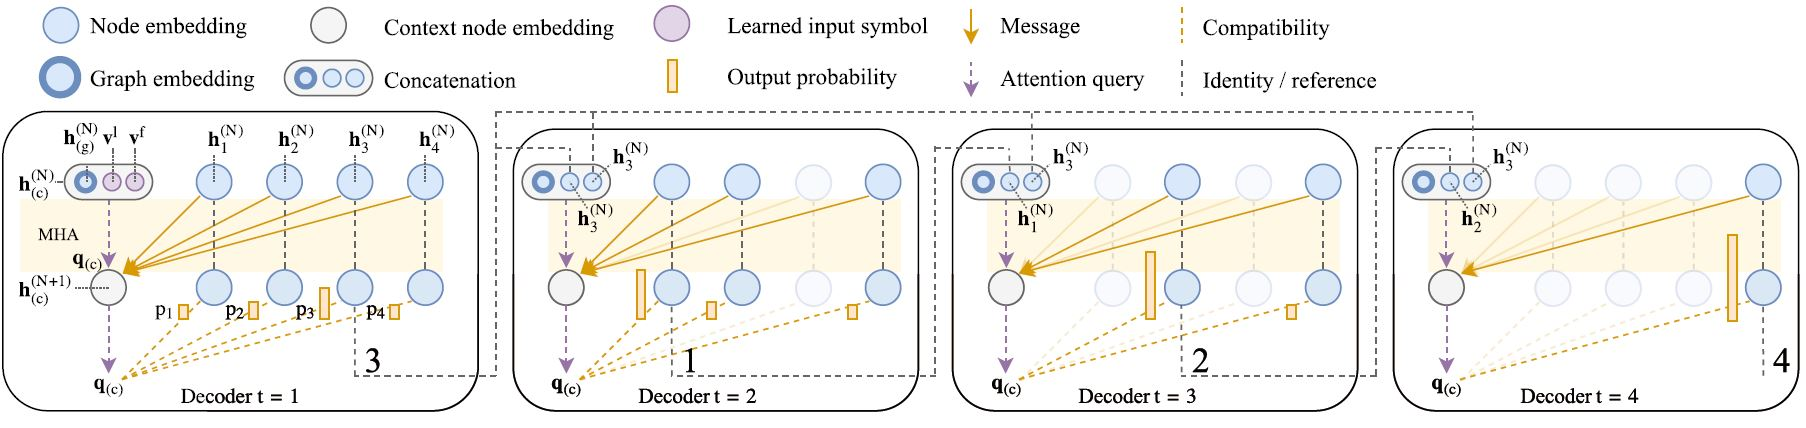
\includegraphics[width=0.99\textwidth]{decoder.jpg}
	\caption{解码器示意图}
	\label{fig:decoder}
\end{figure}

根据内容嵌入计算访问的各个节点成为要访问的下一节点的的概率分布。
\begin{equation}
	q (c)=W^{Q} h _{(c)} \quad k _{i}=W^{K} h _{i}, \quad v _{i}=W^{V} h _{i}
\end{equation}

\textbf{对数概率}\quad
在时间t不能访问的节点,也就是以及访问过的节点,我们通过遮罩赋值为$-\infty$
\begin{equation}
	u_{(c) j}=\left\{\begin{array}{ll}
		C \cdot \tanh \left(\frac{ q _{(c)}^{T} k _{j}}{\sqrt{d_{k}}}\right) & \text { if } j \neq \pi_{t^{\prime}} \quad \forall t^{\prime}<t \\
		-\infty & \text { 其他. }
		\end{array}\right.
\end{equation}

对所有节点的的$u_{(c) j}$通过softmax层,如图\ref{fig:softmax},变换为访问的概率值。

\begin{equation}
	p_{i}=p_{ \theta }\left(\pi_{t}=i \mid s, \pi_{1: t-1}\right)=\frac{e^{u_{(c) t}}}{\sum_{j} e^{u_{(c) \jmath}}}
\end{equation}
\begin{figure}[!h]
	\centering
	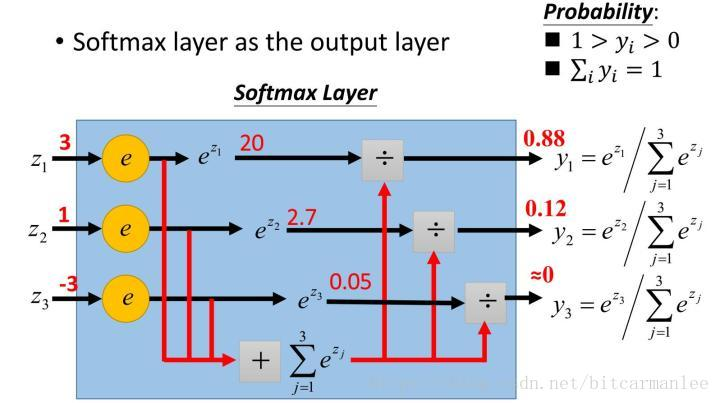
\includegraphics[width=0.6\textwidth]{softmax.jpg}
	\caption{softmax示意图}
	\label{fig:softmax}
\end{figure}
网络的搭建到此结束,我们通过编码器编码场上节点的位置信息,解码器考虑以访问的节点进行内容嵌入,借鉴自然语言处理的注意力机制进行序列式的策略(下一步选取哪个节点访问)输出,最后通过softmax层将模型输出归一化为概率值。

\subsubsection{在贪婪策略的基准线上进行强化学习}
我们以及基于注意的编解码器模型给出策略的计算方法。整个问题实例$s$的解是一系列策略$p(\pi|s)$的序列,也就是说,模型的输出定义了一个所有可能策略的概率分布。
\begin{equation}
	p_{\theta}(\pi \mid s)=\prod_{t=1}^{n} p_{ \theta }\left(\pi_{t} \mid s, \pi_{1: t-1}\right).
\end{equation}
其中模型的所有参数总称为$\theta$。模型的训练过程需要对策略的质量进行评价,我们通过损失函数$L(\pi)$来描述策略的质量。$L(\pi)$定义为路径的总长度。但是不同的问题实例$s$的难度不同,为了使得模型对参数的更新不受问题实例的难易程度影响,我们需要一个基准线。在本模型中,我们使用贪婪策略为基准线
\begin{equation}
	\nabla L ( \theta \mid s)= E _{p_{ \theta }( \pi \mid s)}\left[(L( \pi )-b(s)) \nabla \log p_{ \theta }(\pi \mid s)\right]
\end{equation}
基线$b(s)$的目标是估计实例的难度,这样它就可以联合策略的损失$L(\pi)$共同评价为神经网络提供梯度信息。$b(s)$可以有效降低梯度方差,从而提高学习速度。优化器算法方面,我们使用Adam优化器对神经网络参数进行更新。


\subsection{模型求解}
我们使用的cvrp\_50模型最大支持求解50个传感器的车辆路径问题(VRP)。采用如表\ref{tab:hyper_parameter}所示的超参数训练了100个epoch。
% Table generated by Excel2LaTeX from sheet 'Sheet1'
\begin{table}[htbp]
	\centering
	\caption{Add caption}
	  \begin{tabular}{rrrrrr}
	  \toprule
	  \multicolumn{1}{l}{batch\_size} & \multicolumn{1}{l}{编码器层数} & \multicolumn{1}{l}{exp\_beta} & \multicolumn{1}{l}{model学习率} & \multicolumn{1}{l}{critic学习率} & \multicolumn{1}{l}{梯度修剪阈值} \\
	  \midrule
	  512   & 3     & 0.8   & 0.0001 & 0.0002 & 1 \\
	  \bottomrule
	  \end{tabular}%
	\label{tab:hyper_parameter}%
  \end{table}%

训练过程中,验证集与最优解的差距和epoch的关系如图\ref{fig:trainprocess}所示。

\begin{figure}[!h]
	\centering
	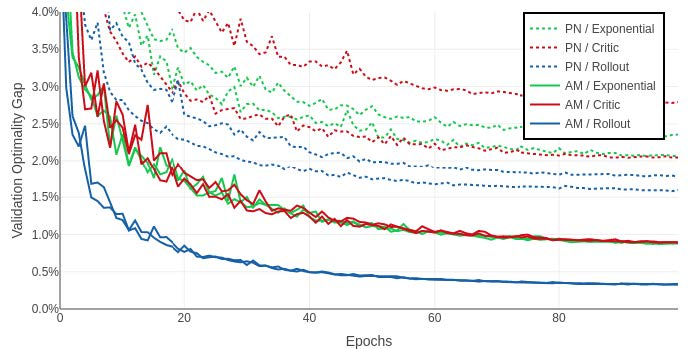
\includegraphics[width=0.9\textwidth]{trainprocess.jpg}
	\caption{训练过程}
	\label{fig:trainprocess}%
\end{figure}
\begin{figure}[H]
	\begin{minipage}[t]{0.45\textwidth}
		\centering
		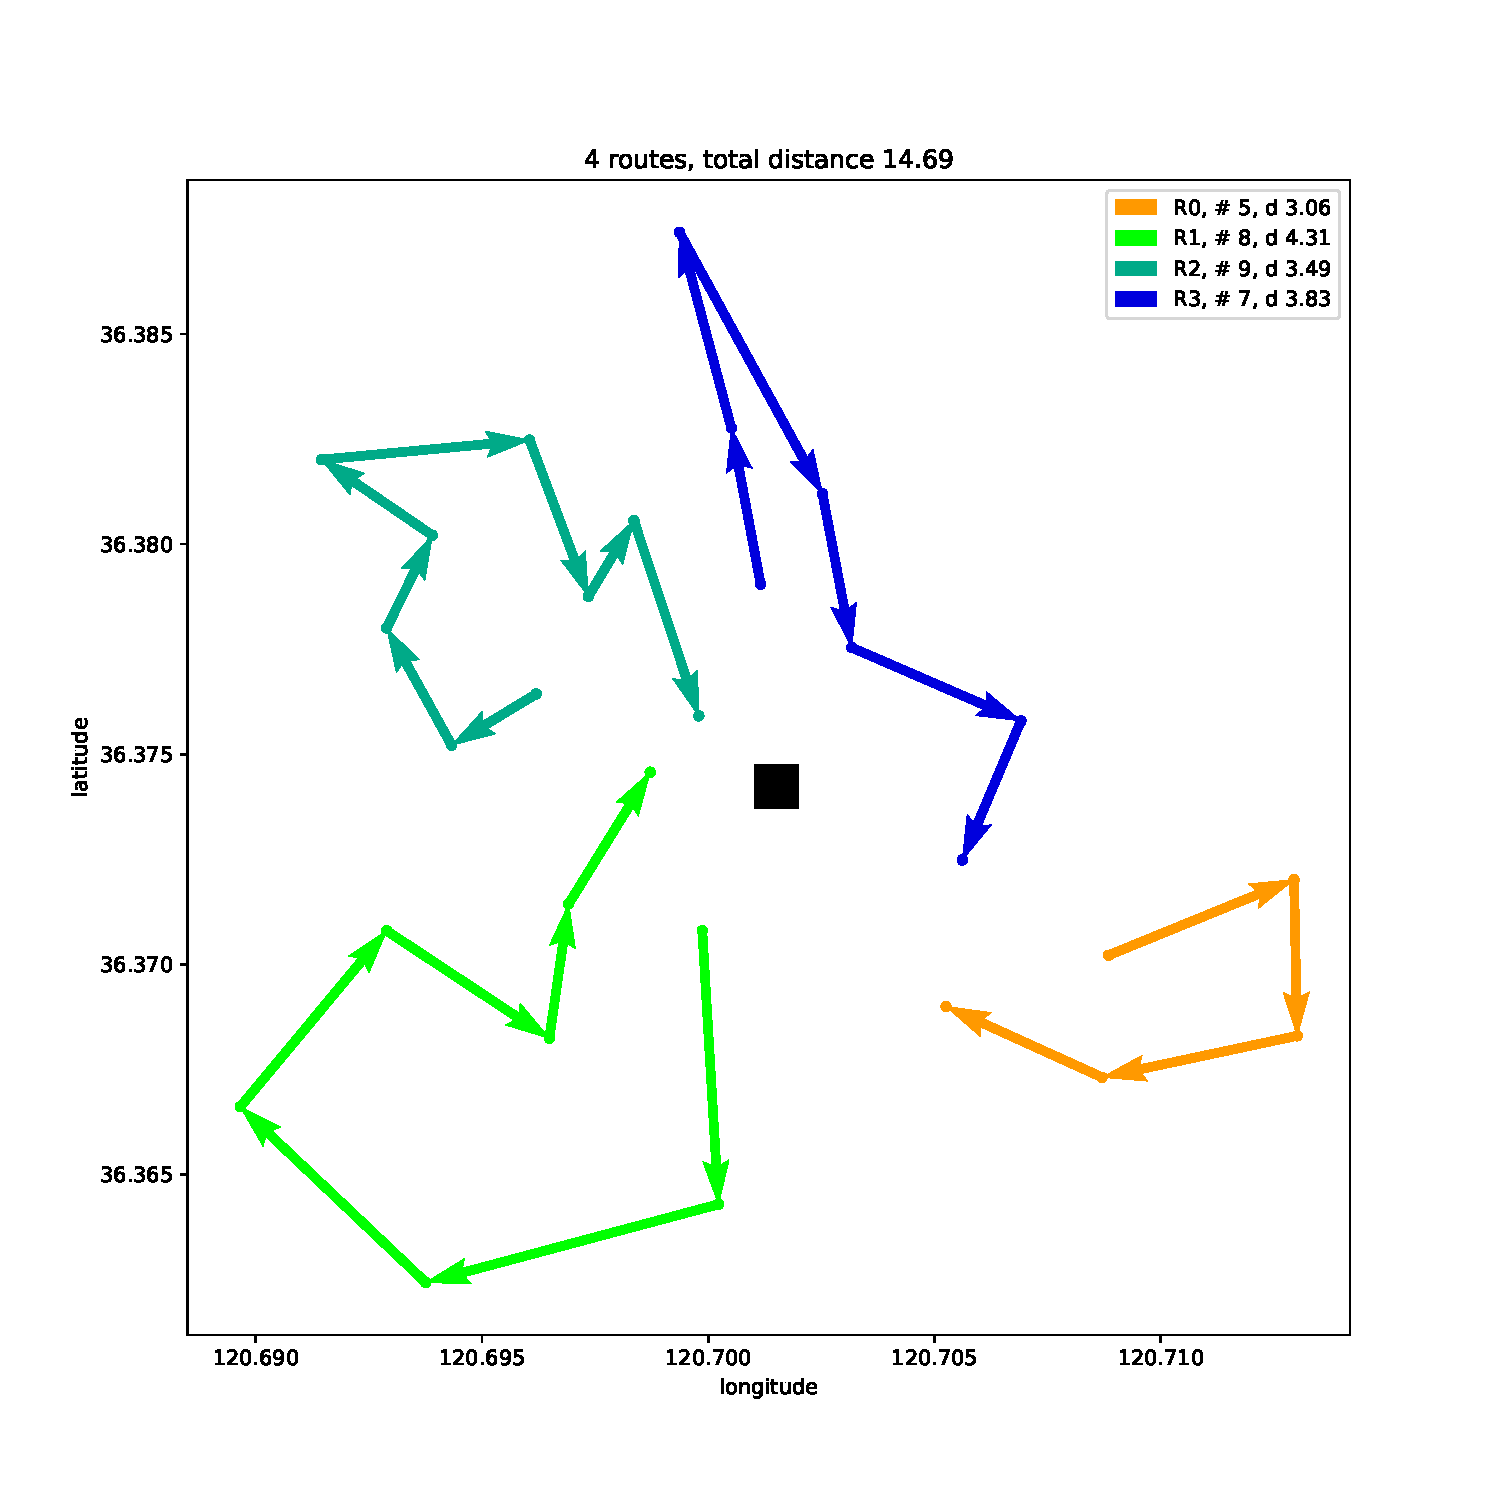
\includegraphics[width=0.99\textwidth]{cvrp_result03.pdf}	
		\label{fig:cvrp_result03_1}
           \caption{平面路径示意}
	\end{minipage}
	\qquad
	\begin{minipage}[t]{0.45\textwidth}
		\centering
		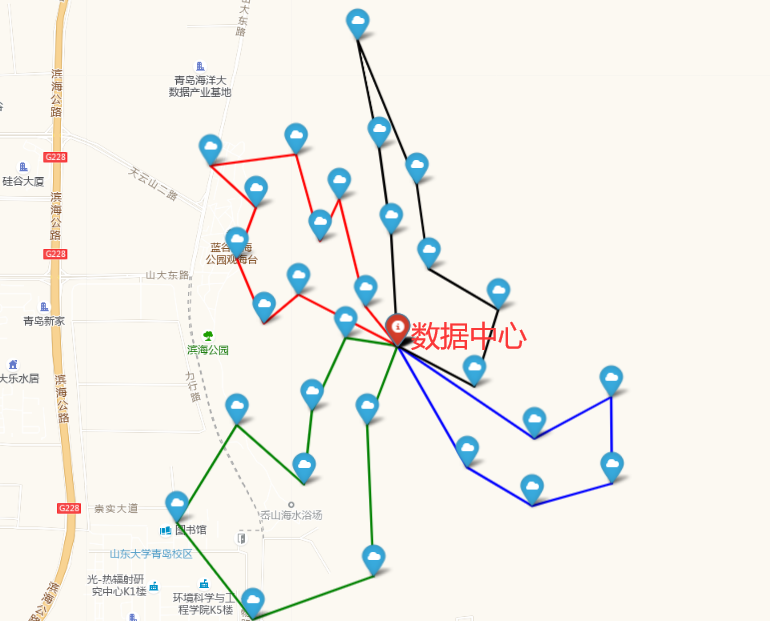
\includegraphics[width=0.99\textwidth]{cvrp_result03.png}
		\label{fig:cvrp_result03_2}
          \caption{三维地图路径示意}	
	\end{minipage}
\end{figure}

% Table generated by Excel2LaTeX from sheet 'Sheet1'
\begin{table}[htbp]
	\centering
	\caption{4辆充电车的路径长度和总长度}
	  \begin{tabular}{rrrrr}
	  \toprule
	  \multicolumn{1}{l}{R0} & \multicolumn{1}{l}{R1} & \multicolumn{1}{l}{R2} & \multicolumn{1}{l}{R3} & \multicolumn{1}{l}{总长} \\
	  \midrule
	  3.06  & 4.31  & 3.49  & 3.83  & 14.69 \\
	  \bottomrule
	  \end{tabular}%
	\label{tab:cvrp_result03}%
  \end{table}%
模型输出的4辆充电车分别的路径长度和总长度见表\ref{tab:cvrp_result03}。

\subsection{灵敏度分析}
我们使用的神经网络模型原本是解决含载重量的车辆路径问题(CVRP)。原始问题中给定了车辆有一个最大的载重量$D$,每一个节点$i \in \{1,2,...,n\}$d,都有一个需求量$\delta$,满足$0<\delta<D$
对于任何一条路径,载重量约束要求。CVRP本身并不支持给的车辆数,而是根据$D$和$\delta$求解出需要的车辆数。
\begin{equation}
	\sum_{i \in R_{j}} \delta_{i} \leq D
	\label{equation:weight_constraint}
\end{equation}
我们使用的预训练模型cvrp\_50训练过程中给定了$D$,而各个传感器节点的需求量$\delta$可以作为数据输入模型。我们调节利用$\delta$使得刚好需要4辆充电车。传感器节点数量$n_M=29$,充电车数量$n_C=4$,为了使得4个充电车每次经过的节点尽量均衡,我们可以利用载重量约束,给定每个节点一个合适的负载。考虑到使负载均衡,我们给所有的传感器节点确定相同的$\delta$。需要强调这个总载重量$D$和节点的需求量$\delta$与题目本身无关,而是车辆路径问题(CVRP)中的要素。$\delta$的值确定如下:
\begin{equation}
	\delta = tolerance\frac{n_C D}{n_M}
\end{equation}
其中$tolerance$是一个0-1之间的参数,表示对负载不均衡的容忍度。因为若取$$\delta = \frac{n_C D}{n_M}$$,则每辆小车必须恰好平均分配节点才能保证每条路径都满足载重量约束,即式\ref{equation:weight_constraint}。
问题三的求解我们使用$\delta=0.1$,可以使得车辆数目为4。我们微调$\delta$观察解的变化。

\begin{figure}[!h]
	\centering
	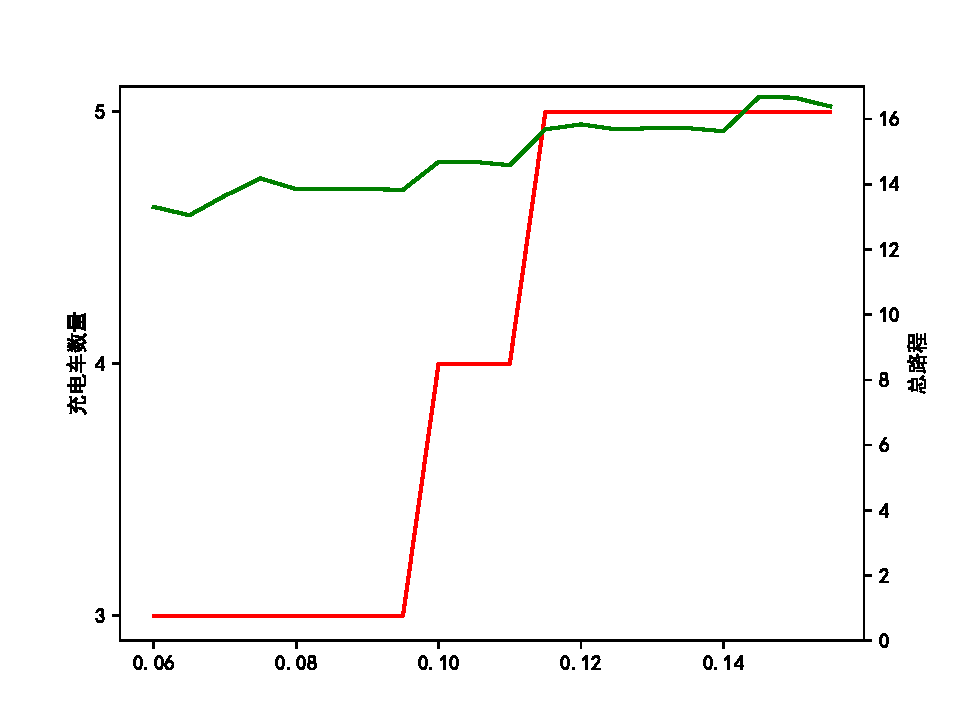
\includegraphics[width=0.6\textwidth]{sensitivity.pdf}
	\caption{车辆数目和总路程对$\delta$的灵敏度}
	\label{fig:sensitivity}%
\end{figure}
可见路径的总长度对于$\delta$不敏感,而小车的数量则敏感依赖$\delta$。这与含载重量的车辆路径问题(CVRP)的特性是相关的,因为在CVRP的设定中,小车数量是给定总载重量$D$和节点的需求量$\delta$后的输出值。我们调节利用$\delta$使得在需要4辆充电车的情况下达到负载均衡。
\newpage

\section{模型评价}

\subsection{模型的优点}
\begin{itemize}
	\item 神经网络模型训练完成后,的推理速度快,在节点规模扩大到小于模型输入参数的维度。
	\item 模型的可推广性强,可以解决车旅行商问题(TSP)、辆路径问题(VRP)、定向问题(OP)和随机问题变体的奖品收集TSP (PCTSP)。
	\item 注意力机制可以利用人类视觉机制进行直观解释。例如,我们的视觉系统倾向于关注图像中辅助判断的部分信息,并忽略掉不相关的信息
\end{itemize}

\subsection{模型的缺点}

\begin{itemize}
	\item 由于模型的最大输入值在训练时就已经确定。所以当节点规模扩大到超出模型输入参数的维度,则需要训练新的模型。
\end{itemize}

\subsection{改进与展望}


\appendix %%附录
%参考文献引用\upcite{bib:one,bib:two}
\begin{thebibliography}{9}%宽度9
	\bibitem{bib:one}崔梦瑶. 可充电无线传感器网络的充电规划设计[D].吉林大学,2018.
	\bibitem{bib:two}吕杨. 无线可充电传感器网络充电规划研究[D].吉林大学,2017.
	\bibitem{bib:three}俞立春. 智能电网中无线可充电传感器网络充电规划研究[D].上海电机学院,2019.
     \bibitem{bib:four}Oriol Vinyals, Meire Fortunato, and Navdeep Jaitly. Pointer networks[J].. In Advances in NeuralInformation Processing Systems, pp. 2692–2700, 2015.
%	\bibitem{bib:one} 邓纪泽. 农村饮水安全管道铺设线路设计分析[J]. 黑龙江水利科技. 2019. 47(11): 92-95.
%	\bibitem{bib:two} 于博. 浅析自来水供水管道施工技术[J]. 百科论坛电子杂志. 2019.(22): 52.
%	\bibitem{bib:three}Shiono N. Suzuki H. Saruwatari Y. A dynamic programming approach for the pipe network layout problem[J]. European journal of operational research. 2019. 277(1): 52-61.
%	\bibitem{bib:four}昝英飞. A numerical model for pipelaying on nonlinear soil stiffness seabed[J]. 水动力学研究与进展:英文版. 2016. 28(1): 10-22.
%	\bibitem{bib:five}Zhou J. Peng J. Liang G. et al. Layout optimization of tree-tree gas pipeline network[J]. Journal of Petroleum Science and Engineering. 2019. 173: 666-680.
\end{thebibliography}
\section{代码}
\subsection{python源程序}
\lstinputlisting[language=python]{code/demo.py}
\subsection{matlab代码}
\begin{lstlisting}[language=matlab]
clc;
%clear;
%% 
[num]=xlsread('point.xlsx');

m=num(:,1);
x=num(:,3);
y=num(:,4);
gtree=zeros(181,181);
for i=1:181
for j=1:181
cell(i,:)=[x(i),y(i)];
end
end
fprintf("length(m):%d\n",length(m));
fprintf("length(x):%d\n",length(x));
fprintf("length(y):%d\n",length(y));
d=zeros(181,181);
for i=1:181
for j=1:181
d(i,j)=sqrt((x(i)-x(j))^2+(y(i)-y(j))^2);
if (i==1&&j>=14) || (j==1&&i>=14)
d(i,j)=-1;
end
end
end

% route=Prime(d(2:181,2:181));
route=Prime(d(1:13,1:13));
for i=1:13
for j=1:13
gtree(i,j)=route(i,j);
end
end

route2=Prime2(d(2:181,2:181),route(2:13,2:13));
for i=2:181
for j=2:181
gtree(i,j)=route2(i-1,j-1);
end
end

%画线路图
scatter(x(1),y(1),'bo')  %中心供水站位置
hold on;
scatter(x(2:13),y(2:13),'k*')  %一级供水站位置
hold on;
scatter(x(14:181),y(14:181),'b.')   %二级供水站位置
hold on;

xlabel('x')
ylabel('y')
% gplot(route,cell(2:181,:),'r-');
gplot(route,cell(1:13,:),'b-')
gplot(route2,cell(2:181,:),'r-')
for i=1:181%length(cell)
%     t=cell(i:181,:);
text(x(i),y(i),[num2str(i)],'color','black','FontSize',10);
end
hleg=legend('中心供水站','一级供水站','二级供水站','一级管道','二级管道','Location','NorthEastOutside');
hold on;
\end{lstlisting}
\end{document}